\chapter[Energia]{Energia}
    \section[Casos de Teste]{Casos de Teste}
        \subsection[NoBreak]{NoBreak}
            \subsubsection[Retificador]{Retificador}
                \begin{itemize}
                    \item \textbf{Pré Condição}:
                        \begin{itemize}
                            \item Tensão 220v Alternada;
                            \item Frequência 60Hz
                        \end{itemize}
                    \item \textbf{Entrada}:
                    \item \textbf{Saída}: Tensão 12v Contínuo
                    \item \textbf{Fluxo de Eventos}: Transformação para 16v alternada; 
                        Retificação por diodos; Carga capacitiva para diminuição de
                        Ripple; Diodo Zener para regulação de Tensão.
                \end{itemize}

            \subsubsection[Inversor]{Inversor}
                \begin{itemize}
                    \item \textbf{Pré Condição}: Tensão 12V contínua
                    \item \textbf{Entrada}:
                    \item \textbf{Saída}: 
                        \begin{itemize}
                            \item Frequência 60Hz
                            \item Tensão 220v Alternada
                        \end{itemize}
                    \item \textbf{Fluxo de Eventos}: Chaveamento  de Transistores em ciclos 
                        diferentes (60Hz); Transformação de 12+12v para 220v Alternado.
                \end{itemize}
                            
        \subsection[Refrigeração]{Refrigeração}
            \subsubsection[Chiller]{Chiller}
                \begin{itemize}
                    \item \textbf{Pré Condição}:
                    \item \textbf{Entrada}:
                    \item \textbf{Saída}: 
                    \item \textbf{Fluxo de Eventos}:
                \end{itemize}

        \section[Sistema de Refrigeração]{Sistema de Refrigeração}

            Na parte de planejamento do sistema de refrigeração, foram feitos todos os
            cálculos referentes ao sistema. Para o cálculo do tamanho da serpentina (perguntar
            gabriela) Colocar tbm a vazão de retirada do chopp

            O dimensionamento da potência do compressor, necessário no ciclo de
            refrigeração foi feito a partir da Primeira Lei da Termodinâmica, onde calculou-se a
            carga térmica necessária a ser retirada do chopp, considerando que a vazão
            necessária a ser retirada da chopeira é 45l/h, ou aproximadamente, 0,00125m$^3$/s, a
            Primeira Lei para o compressor será:
            
            \begin{equation}
                Q_{(ponto)} = m_{(ponto)} \times (h_1 - h_2)
            \end{equation}

            Onde:
            \begin{itemize}
                \item Q = Quantidade de calor
                \item m = fluxo mássico (vazão multiplicada pela densidade)
                \item h = entalpia
            \end{itemize}
            
            Manipulando, têm-se:

            \begin{equation}
                h_1 - h_2 = Cp_{méd} \times (T_1 - T_2)
            \end{equation}

            Onde:
            \begin{itemize}
                \item $Cp_{médi}$ = Calor Específico a pressão constante
                \item T = Temperatura do fluido
            \end{itemize}
            então, substituindo na primeira equação teremos:

            \begin{equation}
                Q_{ponto} = m_{ponto} \times Cp_{méd} \times (T_1 - T_2)
            \end{equation}

            Consideramos como fluido para os cálculos a água, visto que o chopp tem bastante 
            água na sua composição e que não foram encontrados dados para o calor específico 
            do chopp, a aproximação é aceitável. O valor de calor específico a pressão constante
            encontrado para a água é de 4,18KJ/Kg. A temperatura considerada na entrada do 
            trocador de calor é a mesma que a temperatura ambiente de aproximadamente 25$\circ$C,
            e a requerida na saída dele para estar de acordo com os requisitos é de
            aproximadamente 1$\circ$C. Dessa forma, o fluxo mássico

            \begin{equation}
                m_{ponto} = p \times V
            \end{equation}

            \begin{equation}
                m_{ponto} = 1000 \times 0,00125
            \end{equation}

            \begin{equation}
                m_{ponto} = 0,0125
            \end{equation}

            Logo, a carga térmica a ser retirada do fluido, no trocador de calor,
            pelo gás que sai do compressor será:
            
            \begin{equation}
                Q_{ponto} = 0.0125 \times 4.18 \times (25-1(-1)) = 1.35 KW
            \end{equation}

            Ou então:
            \begin{equation}
                46.32.48 Btu/h
            \end{equation}

            Analisando o catálogo (nome), para essa carga térmica seria necessário um compressor de
            $1 \over 2$ Hp. Colocar print do catálogo

            \subsubsection[Simulação do sistema de Refrigeração]{Simulação do sistema de Refrigeração}
                Para a segurança do funcionamento do sistema de refrigeração usou-se o
                Software CoolPack para a simulação do sistema como um todo. Nesse
                software dados construtivos físicos dos seguintes elementos foram inseridos: 
                Evaporador, Condensador, moto-compressor e tubulação. 

                A figura seguinte ilustra a simulação realizada no software juntamente com os os
                dados das temperaturas em cada estado. Essas temperaturas serão importantes para o
                devido entendimento da troca de calor entre evaporador e o líquido externo ao
                sistema a ser refrigerado.

                \begin{figure}[!htb]
            		\centering
            		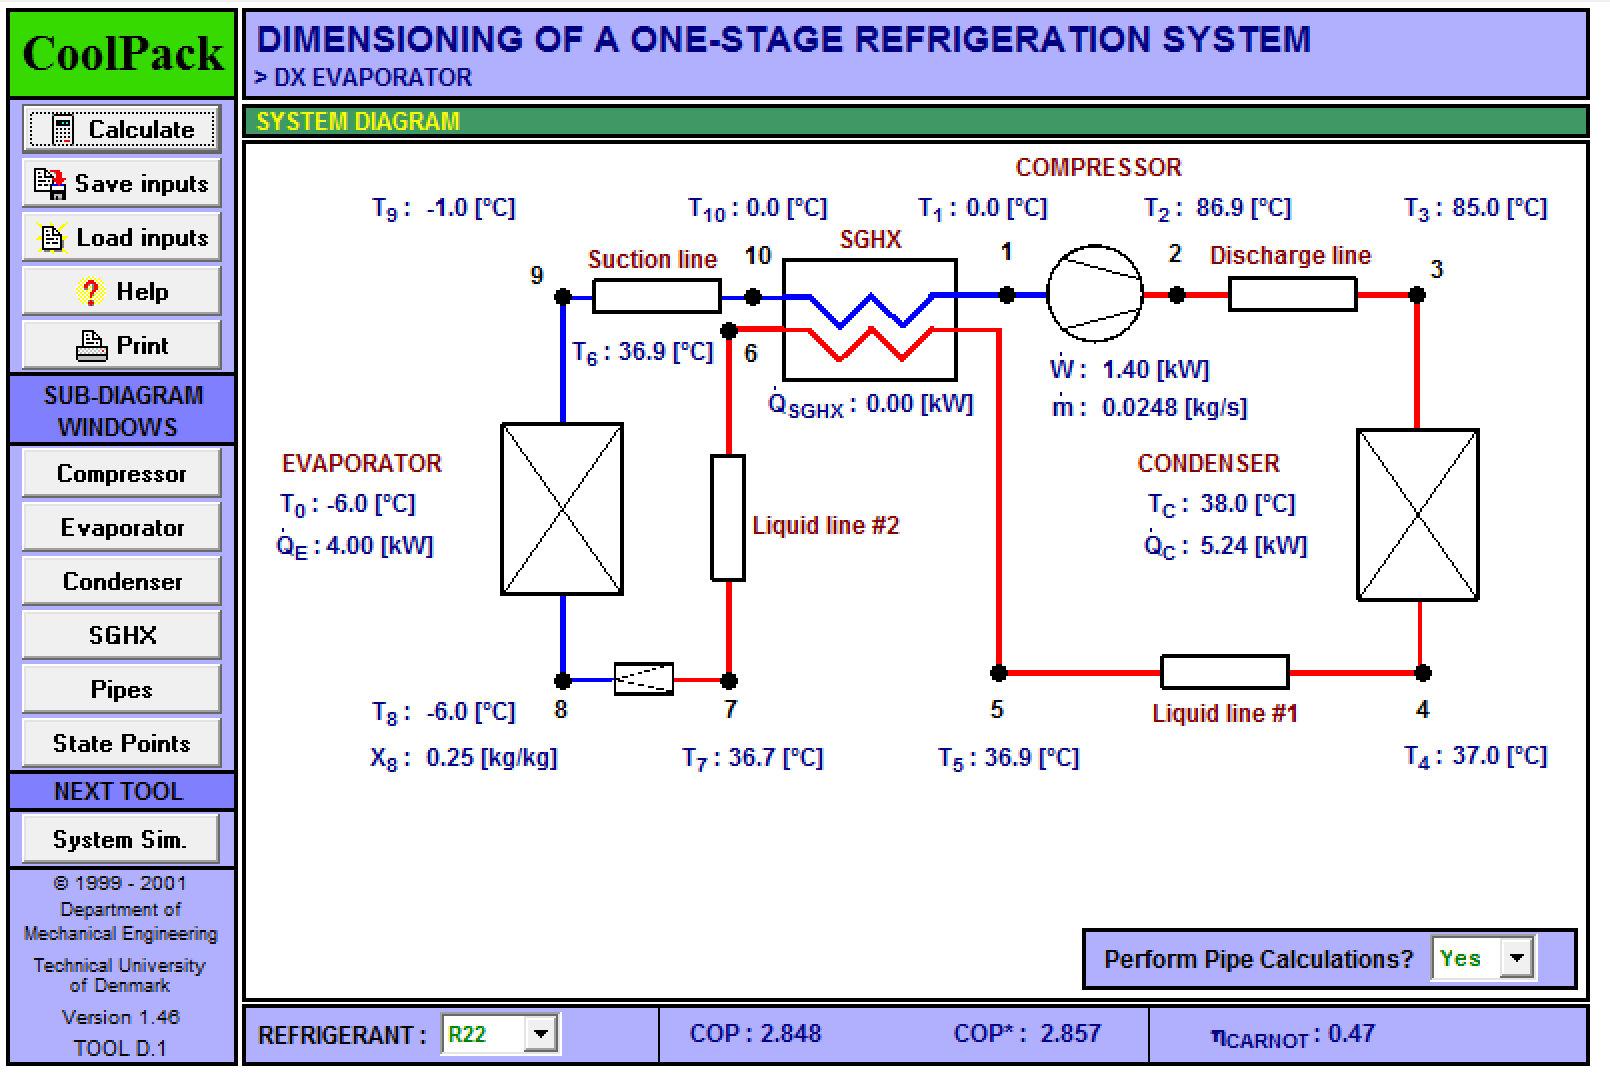
\includegraphics[scale= 0.3]{figuras/simulacao-refrigeracao.png}
            		\caption{Simulação do sistema de Refrigeração. Fonte: Própria.}
            		\label{simulacao-refrigeracao}
            	\end{figure}

                Observa-se na imagem acima que foi inserido o dado correto quanto ao tipo de
                gás em que o compressor opera. Tem-se como resultado importante a quantidade
                de energia, ou seja, calor transferida no evaporador que corresponde a 4.00 kW.
                Esse dado será validado nos testes do sistema já montado

            \subsection[Simulação Chiller]{Simulação Chiller}

            \subsection[Montagem e Construção do Sistema de Refrigeração]{Montagem e Construção do Sistema de Refrigeração}
                A montagem foi feita com apenas um chirller no protótipo por motivos de custo,
                sendo assim, a potência do compressor foi reduzida pela metade, ou seja, $1 \over 4$ Hp.
                O compressor foi cedido pelo professor Rander, para viabilizar que o protótipo
                fosse fabricado, as especificações desse compressor são as seguintes:

                \begin{figure}[!htb]
            		\centering
            		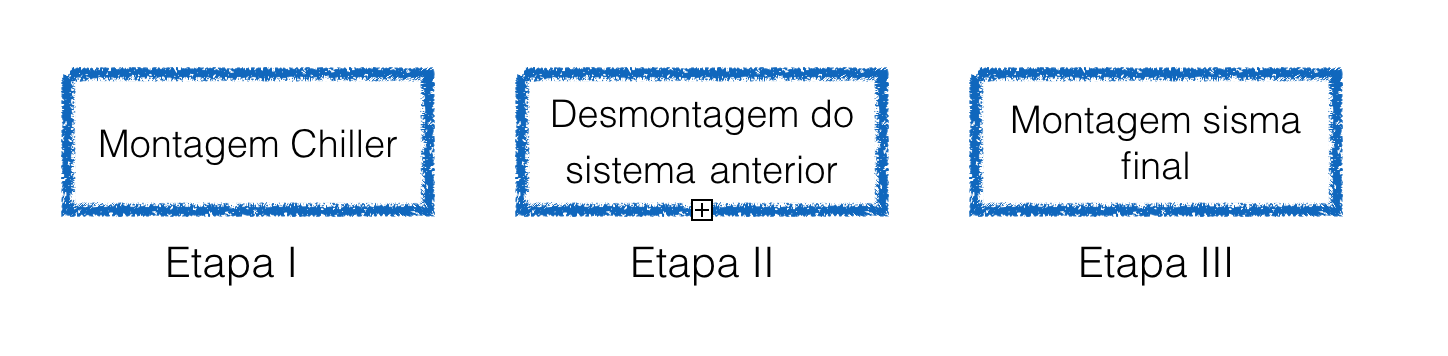
\includegraphics[scale= 0.3]{figuras/montagem-chiler.png}
            		\caption{Processo de Montagem do Sistema de Refrigeração. Fonte: Própria.}
            		\label{simulacao-refrigeracao}
            	\end{figure}
                
                \subsubsection[Descrição das etapas]{Descrição das etapas}
                    Para a montagem do sistema de refrigeração teve que seguir as seguintes etapas:                    
                    \subsubsubsection[Manufaturação do Chirller]{Manufaturação do Chirller}
                        Neste processo, os materiais utilizados foram: uma panqueca de alumínio $3 \over 8$ e
                        15 metros, uma mangueira atóxica trançada $3 \over 4$, 2 kits de engate rápido para
                        mangueira, 2  reduções de $3 \over 4$ para $1 \over 2$, 2 tês de PVC com extremidades de $3 \over 4$
                        e central de $1 \over 2$, 2 espigões de mangueira de $3 \over 4$ e 4 niples de união de $1 \over 2$,
                        2 braçadeiras de $3 \over 4$ e 2 adaptadores de gás de $1 \over 2$ para $3 \over 8$.
                        Primeiro, lavou-se a mangueira com água e sabão, feito isso,
                        desenrolou-se a panqueca em todo o seu comprimento, de forma que ela
                        ficasse bem reta. 
                        
                        Na segunda parte do processo, o tubo de alumínio foi inserido dentro da
                        mangueira, ainda de forma que que a estrutura ficasse reta. Depois,
                        enrolou-se a estrutura no molde, que tem 30cm de diâmetro, prendendo
                        ele com lacres de plástico. A imagem a seguir ilustra esse processo,
                        feito por membros do grupo:

                        \begin{figure}[!htb]
                            \centering
                            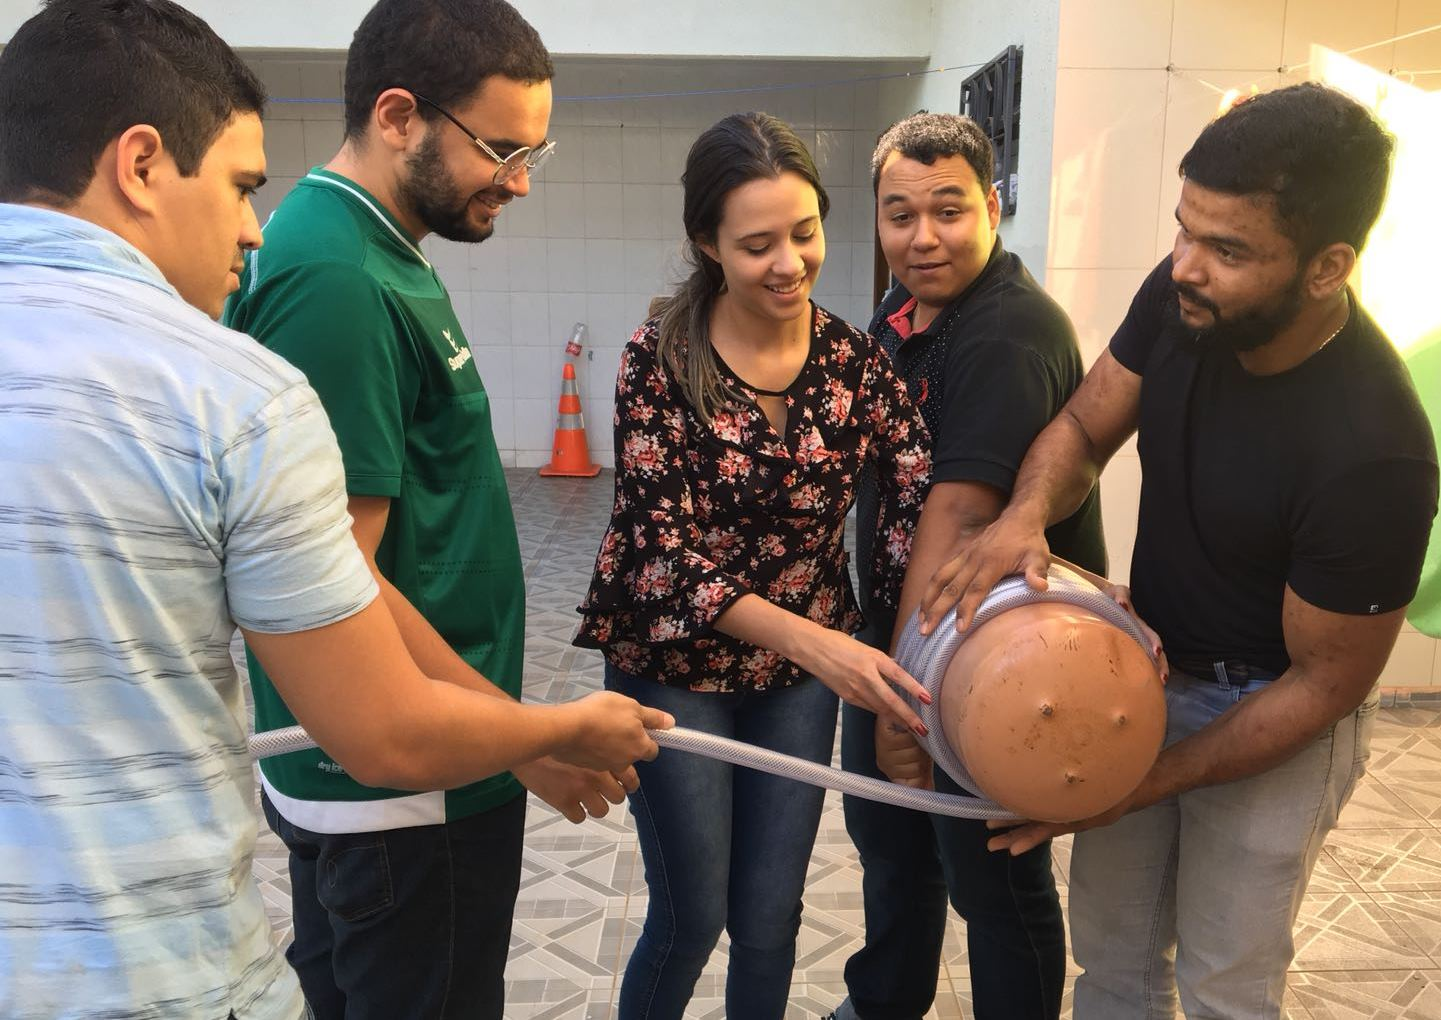
\includegraphics[scale= 0.3]{figuras/moldagem-chiller.png}
                            \caption{Moldagem do chirller. Fonte: Própria.}
                            \label{moldagem-chiller}
                        \end{figure}

                        Foi feito um desenho esquemático do Chirller no software CatiaV5 para
                        possibilitar as simulações, ele está ilustrado na figura xx.

                        \begin{figure}[!htb]
                            \centering
                            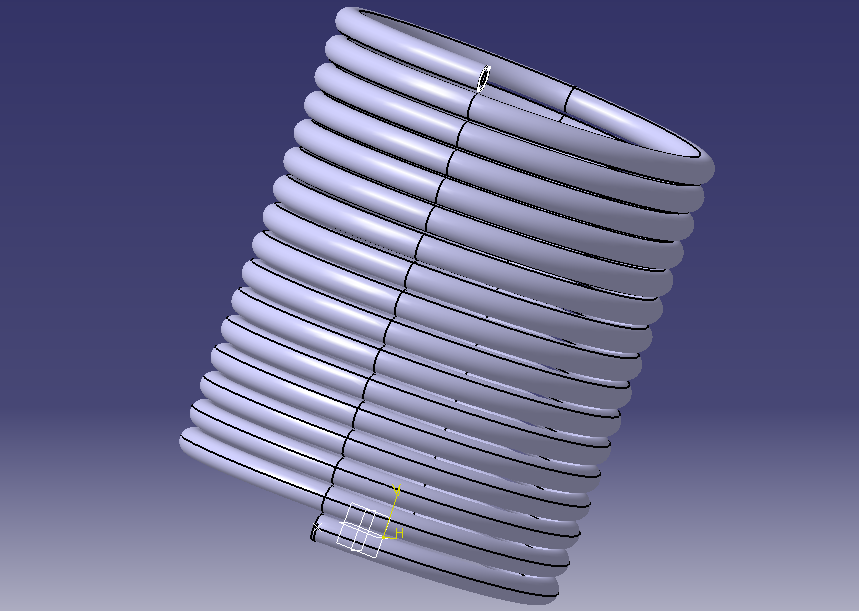
\includegraphics[scale= 0.3]{figuras/desenho-chiller.png}
                            \caption{Desenho esquemático do chirller. Fonte: Própria.}
                            \label{desenho-chiller}
                        \end{figure}

                        \begin{figure}[!htb]
                            \centering
                            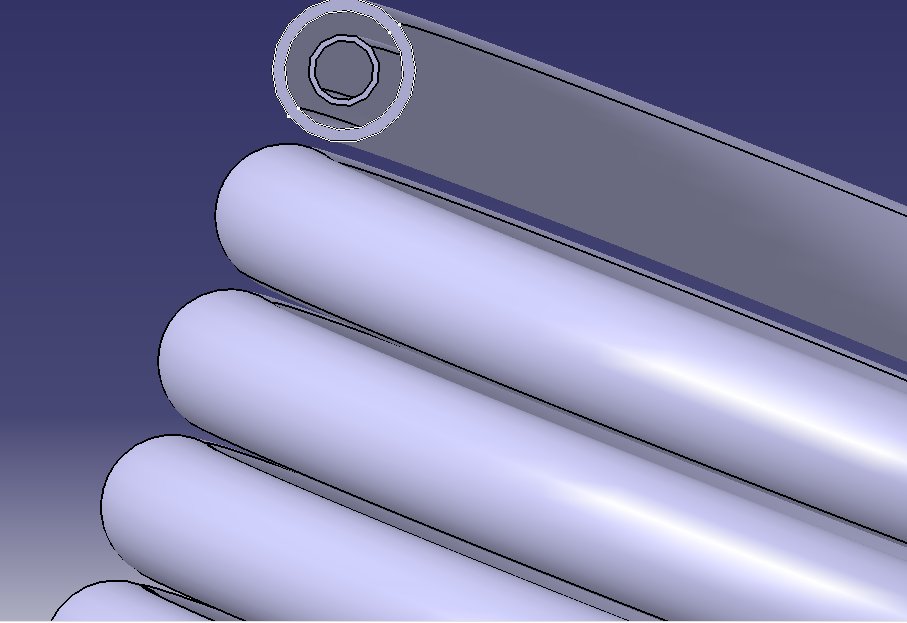
\includegraphics[scale= 0.3]{figuras/corte-mangeira.png}
                            \caption{Vista em corte da mangueira com o tubo de alumínio inserido. Fonte: Própria.}
                            \label{vista-mangueira}
                        \end{figure}

                        Na terceira parte da passagem, passou-se fita veda-rosca em todos os acessórios de
                        tubulação, para evitar vazamentos, e montou-se o tê adaptado que possibilita a
                        entrada e saída de chopp no Chirller de contra-fluxo. Neste processo,
                        coloca-se o espigão em uma extremidade de $3 \over 4$ do tê, um nipple de união
                        de $1 \over 2$ na extremidade de $1 \over 2$ do tê, um engate rápido no nipple. Na outra
                        extremidade de $3 \over 4$, coloca-se uma redução de $3 \over 4$ pra $1 \over 2$, coloca-se
                        um nipple de união e por fim, coloca-se um adaptador de gás no nipple. Depois
                        de montado o tê adaptado ficou da seguinte maneira:

                        \begin{figure}[!htb]
                            \centering
                            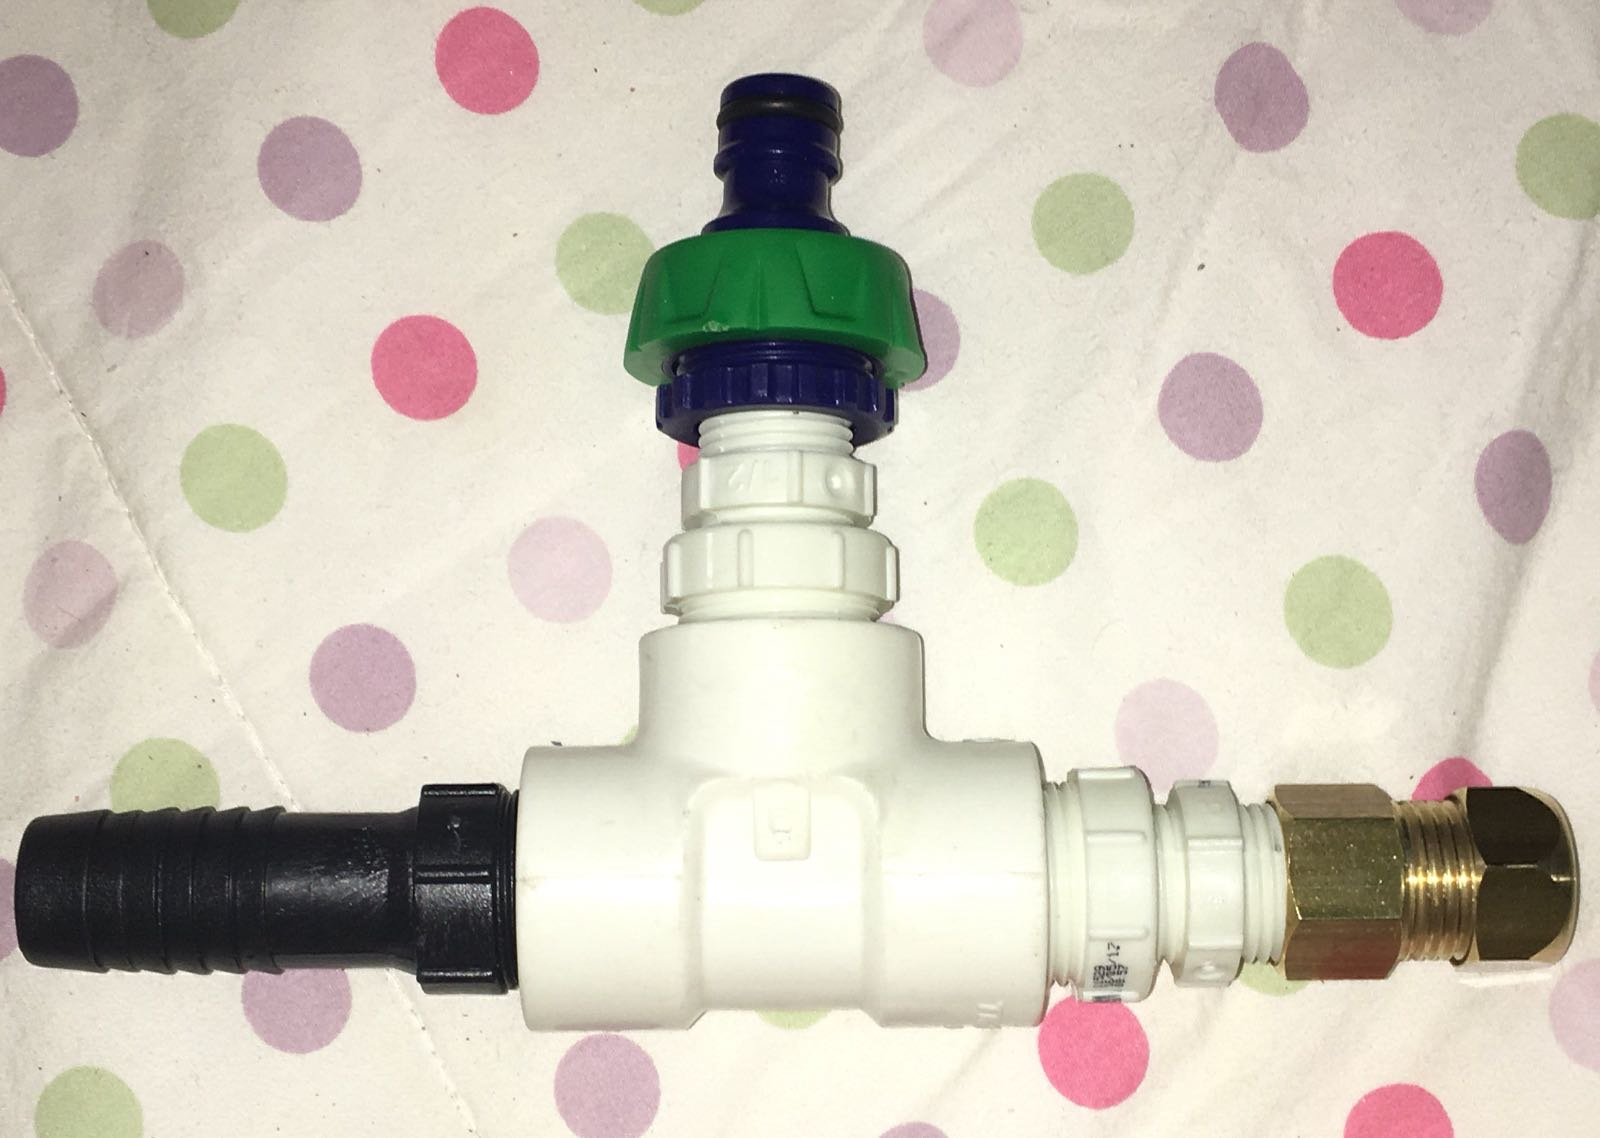
\includegraphics[scale= 0.3]{figuras/entrada-saida-chopp.png}
                            \caption{Tê adaptado para entrada e saída de chopp. Fonte: Própria.}
                            \label{entrada-saida-chopp}
                        \end{figure}

                    \subsubsubsection[Desmontagem do Sistema]{Desmontagem do Sistema}
                        Nessa etapa teve-se o devido cuidado para a desmontagem do sistema. Retirou-se o gás
                        R22 com o equipamento próprio para tal ação, considerando assim a lei ambiental
                        quanto a emissão de gases poluentes na atmosfera. Dessa forma, na válvula
                        de serviço do compressor a válvula de descarga do fluido refrigerante
                        encaminhando-o para o devido recipiente de armazenamento de gás a vacuo.
                        Desse modo realizou-se o procedimento de recolhimento passivo. Esse procedimento e
                        indicado para quantidades pequenas de gas. Ele pode ser retirado na sua forma gasosa
                        ou líquida. Isso acontece devido a diferença de pressão entre os dois sistemas.

                        Esse procedimento foi realizado a fim de atender a Resolução CONAMA no 267, de 14 de
                        setembro de 2000. Essa resolução proíbe a utilização e consequentemente emissão
                        de substâncias que destroem a camada de ozônio. 

                    \subsubsubsection[Montagem do Sistema]{Montagem do Sistema}
                        Após a devida manufatura do Chiller e a desmontagem do sistema escolheu-se uma
                        base e alocou-se os componentes de acordo com a figura \ref{alocacao-dispositivos} 

                        \begin{figure}[!htb]
                            \centering
                            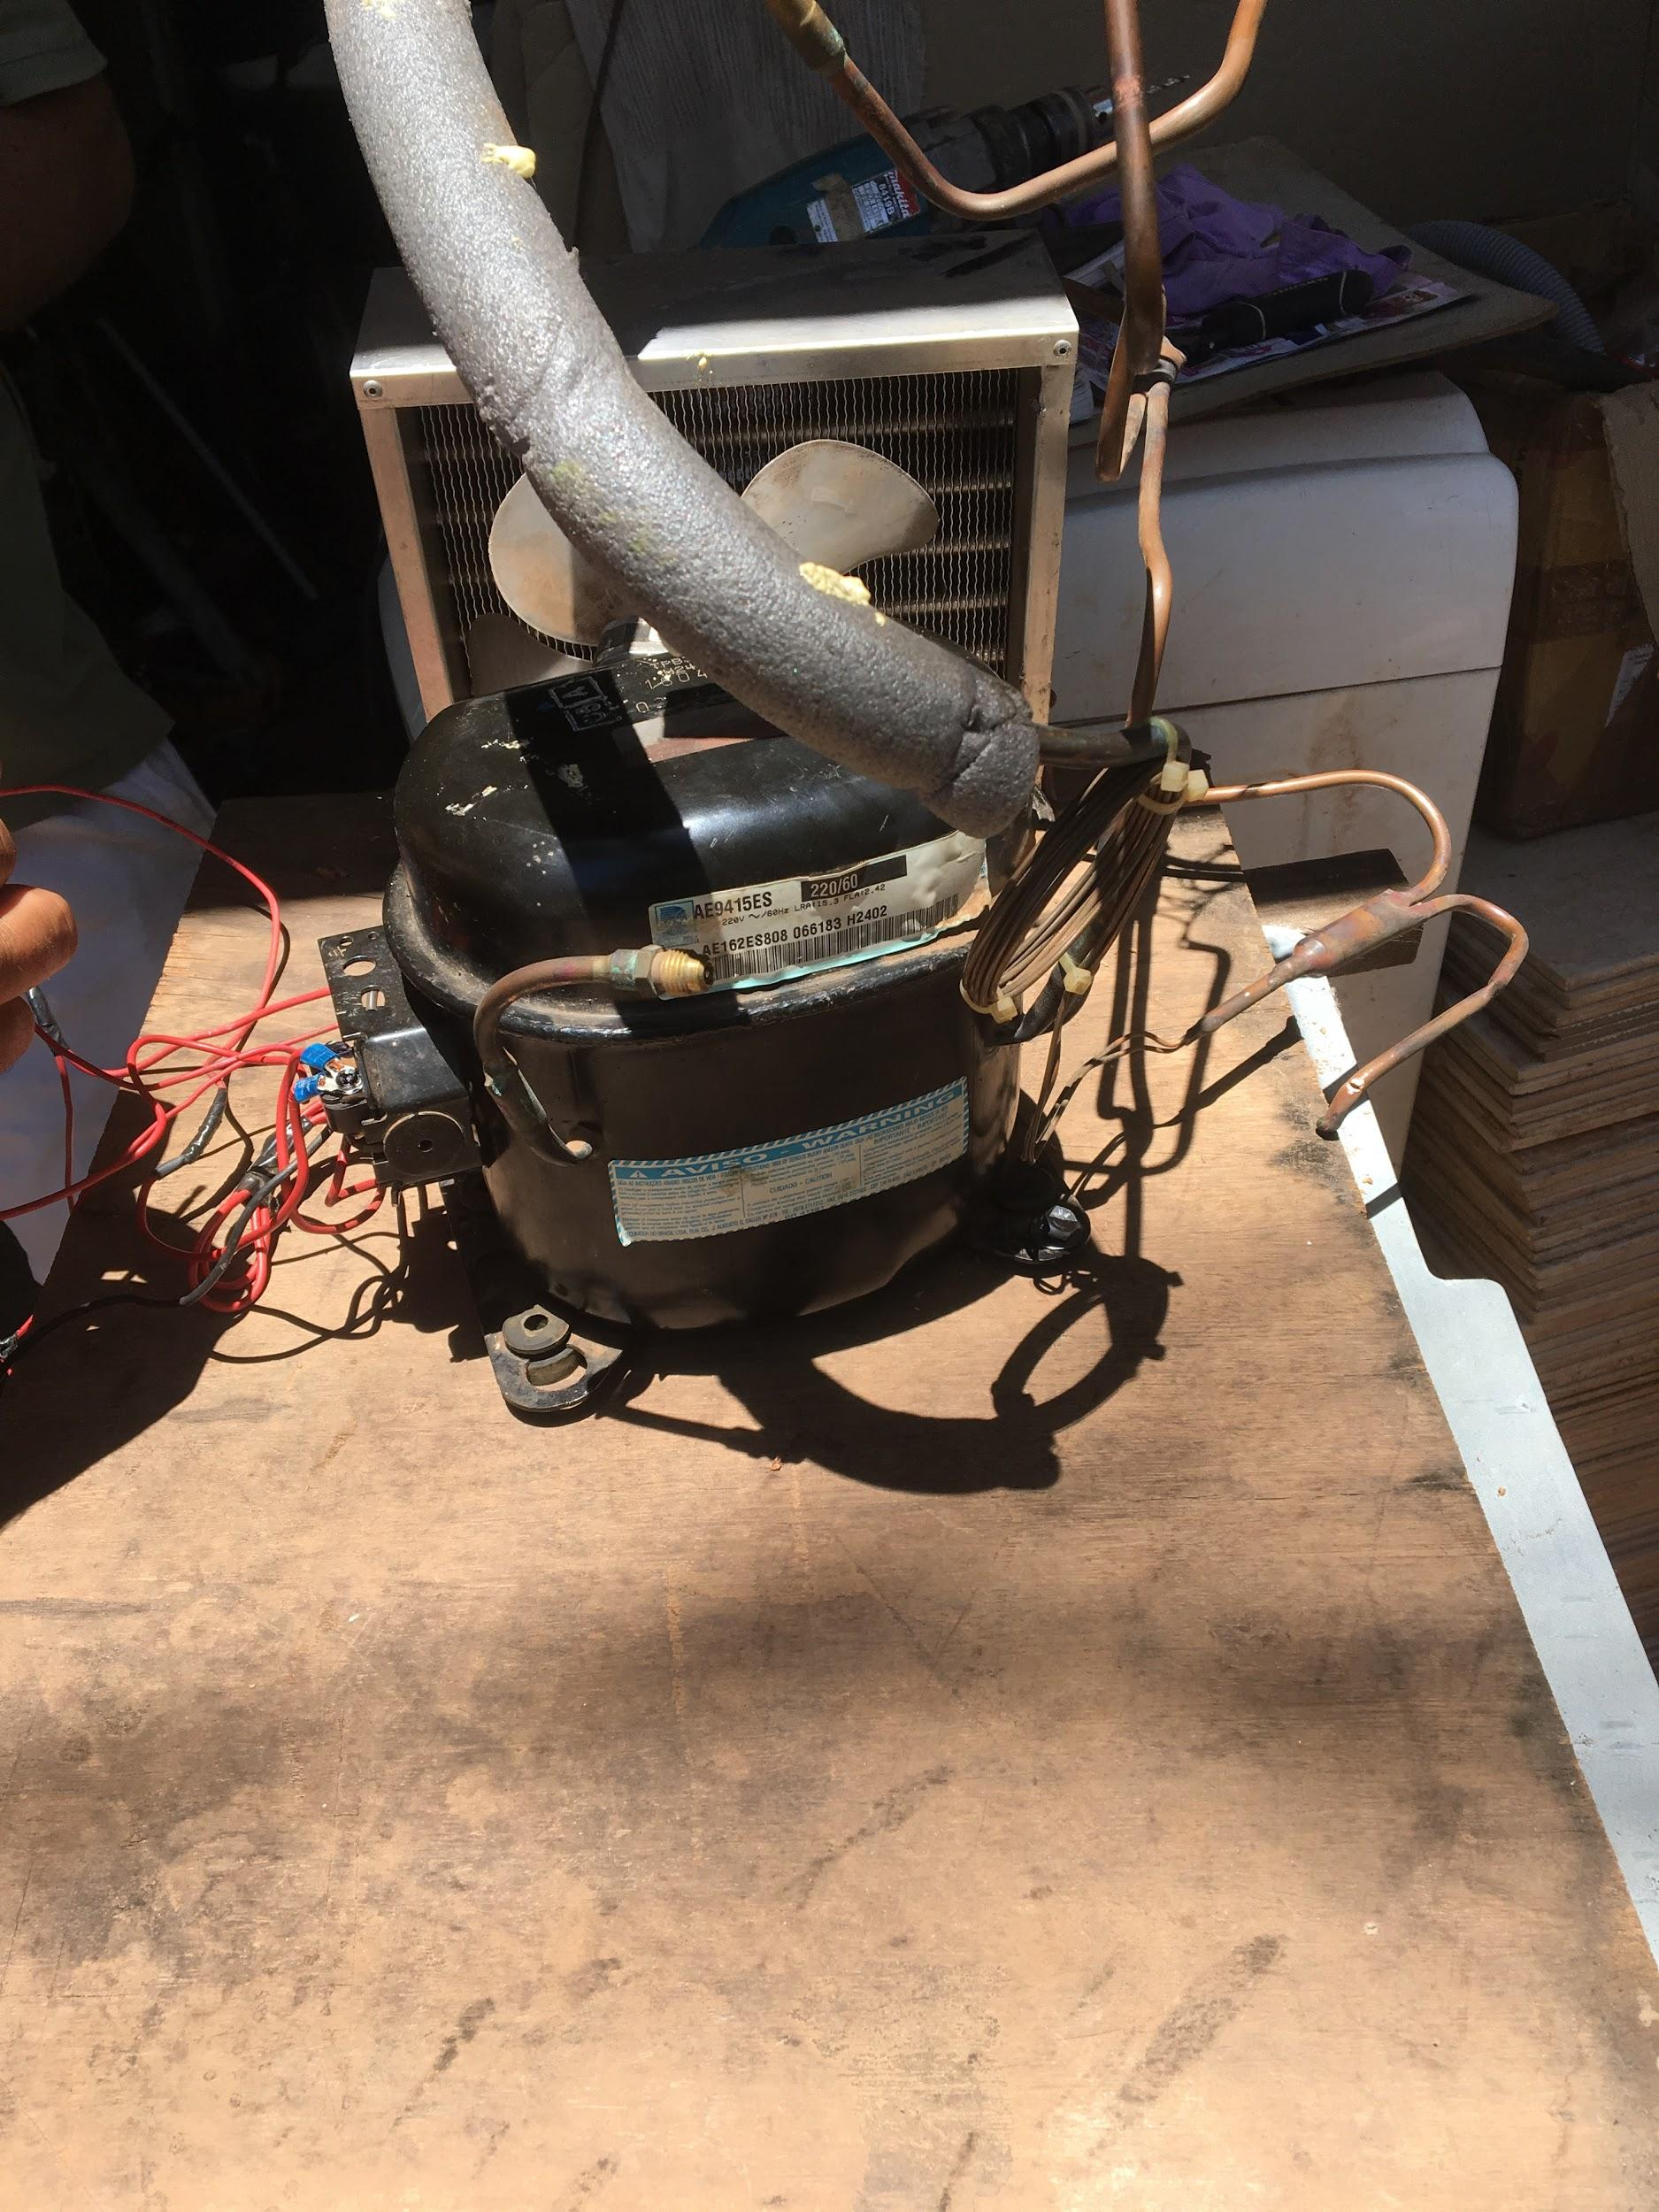
\includegraphics[scale= 0.2]{figuras/alocacao-dispositivos.png}
                            \caption{Sistema aberto e alocação dos dispositivos. Fonte: Própria.}
                            \label{alocacao-dispositivos}
                        \end{figure}

                        A base para o sistema consiste em uma de material madeira. Esse material foi
                        escolhido devido às suas propriedades térmicas e pela fácil disponibilidade desse. 
                        
                        Realizou-se testes de pressão no motocompressor e constatou-se que esse encontrava-se
                        com baixa capacidade de compressão. Sendo assim realizou-se a limpeza do motor e
                        também a troca de do filtro do sistema para o filtro secador do tipo Darfur.
                        Este filtro impede com que partículas indesejadas passem pela a tubulação e cheguem
                        no motocompressor. Além disso, como o filtro secador foi trocado optou-se, por medidas
                        preventivas, trocar o filtro capilar. 

                        COLOCAR FOTO FILTRO DANFUR NO SISTEMA. 

                        A tubulação do Chiller escolhido consiste de alumínio e as demais tubulações do
                        sistema sao de cobre. Assim sendo, tornando inviável a solda desses dispositivos como
                        solução. A partir disso, optou-se pela aquisição da junção de gás (nipel)
                        com a cabeça em forma de cilindro ilustrado na figura \ref{nipel-gas}.
                        
                        \begin{figure}[!htb]
                            \centering
                            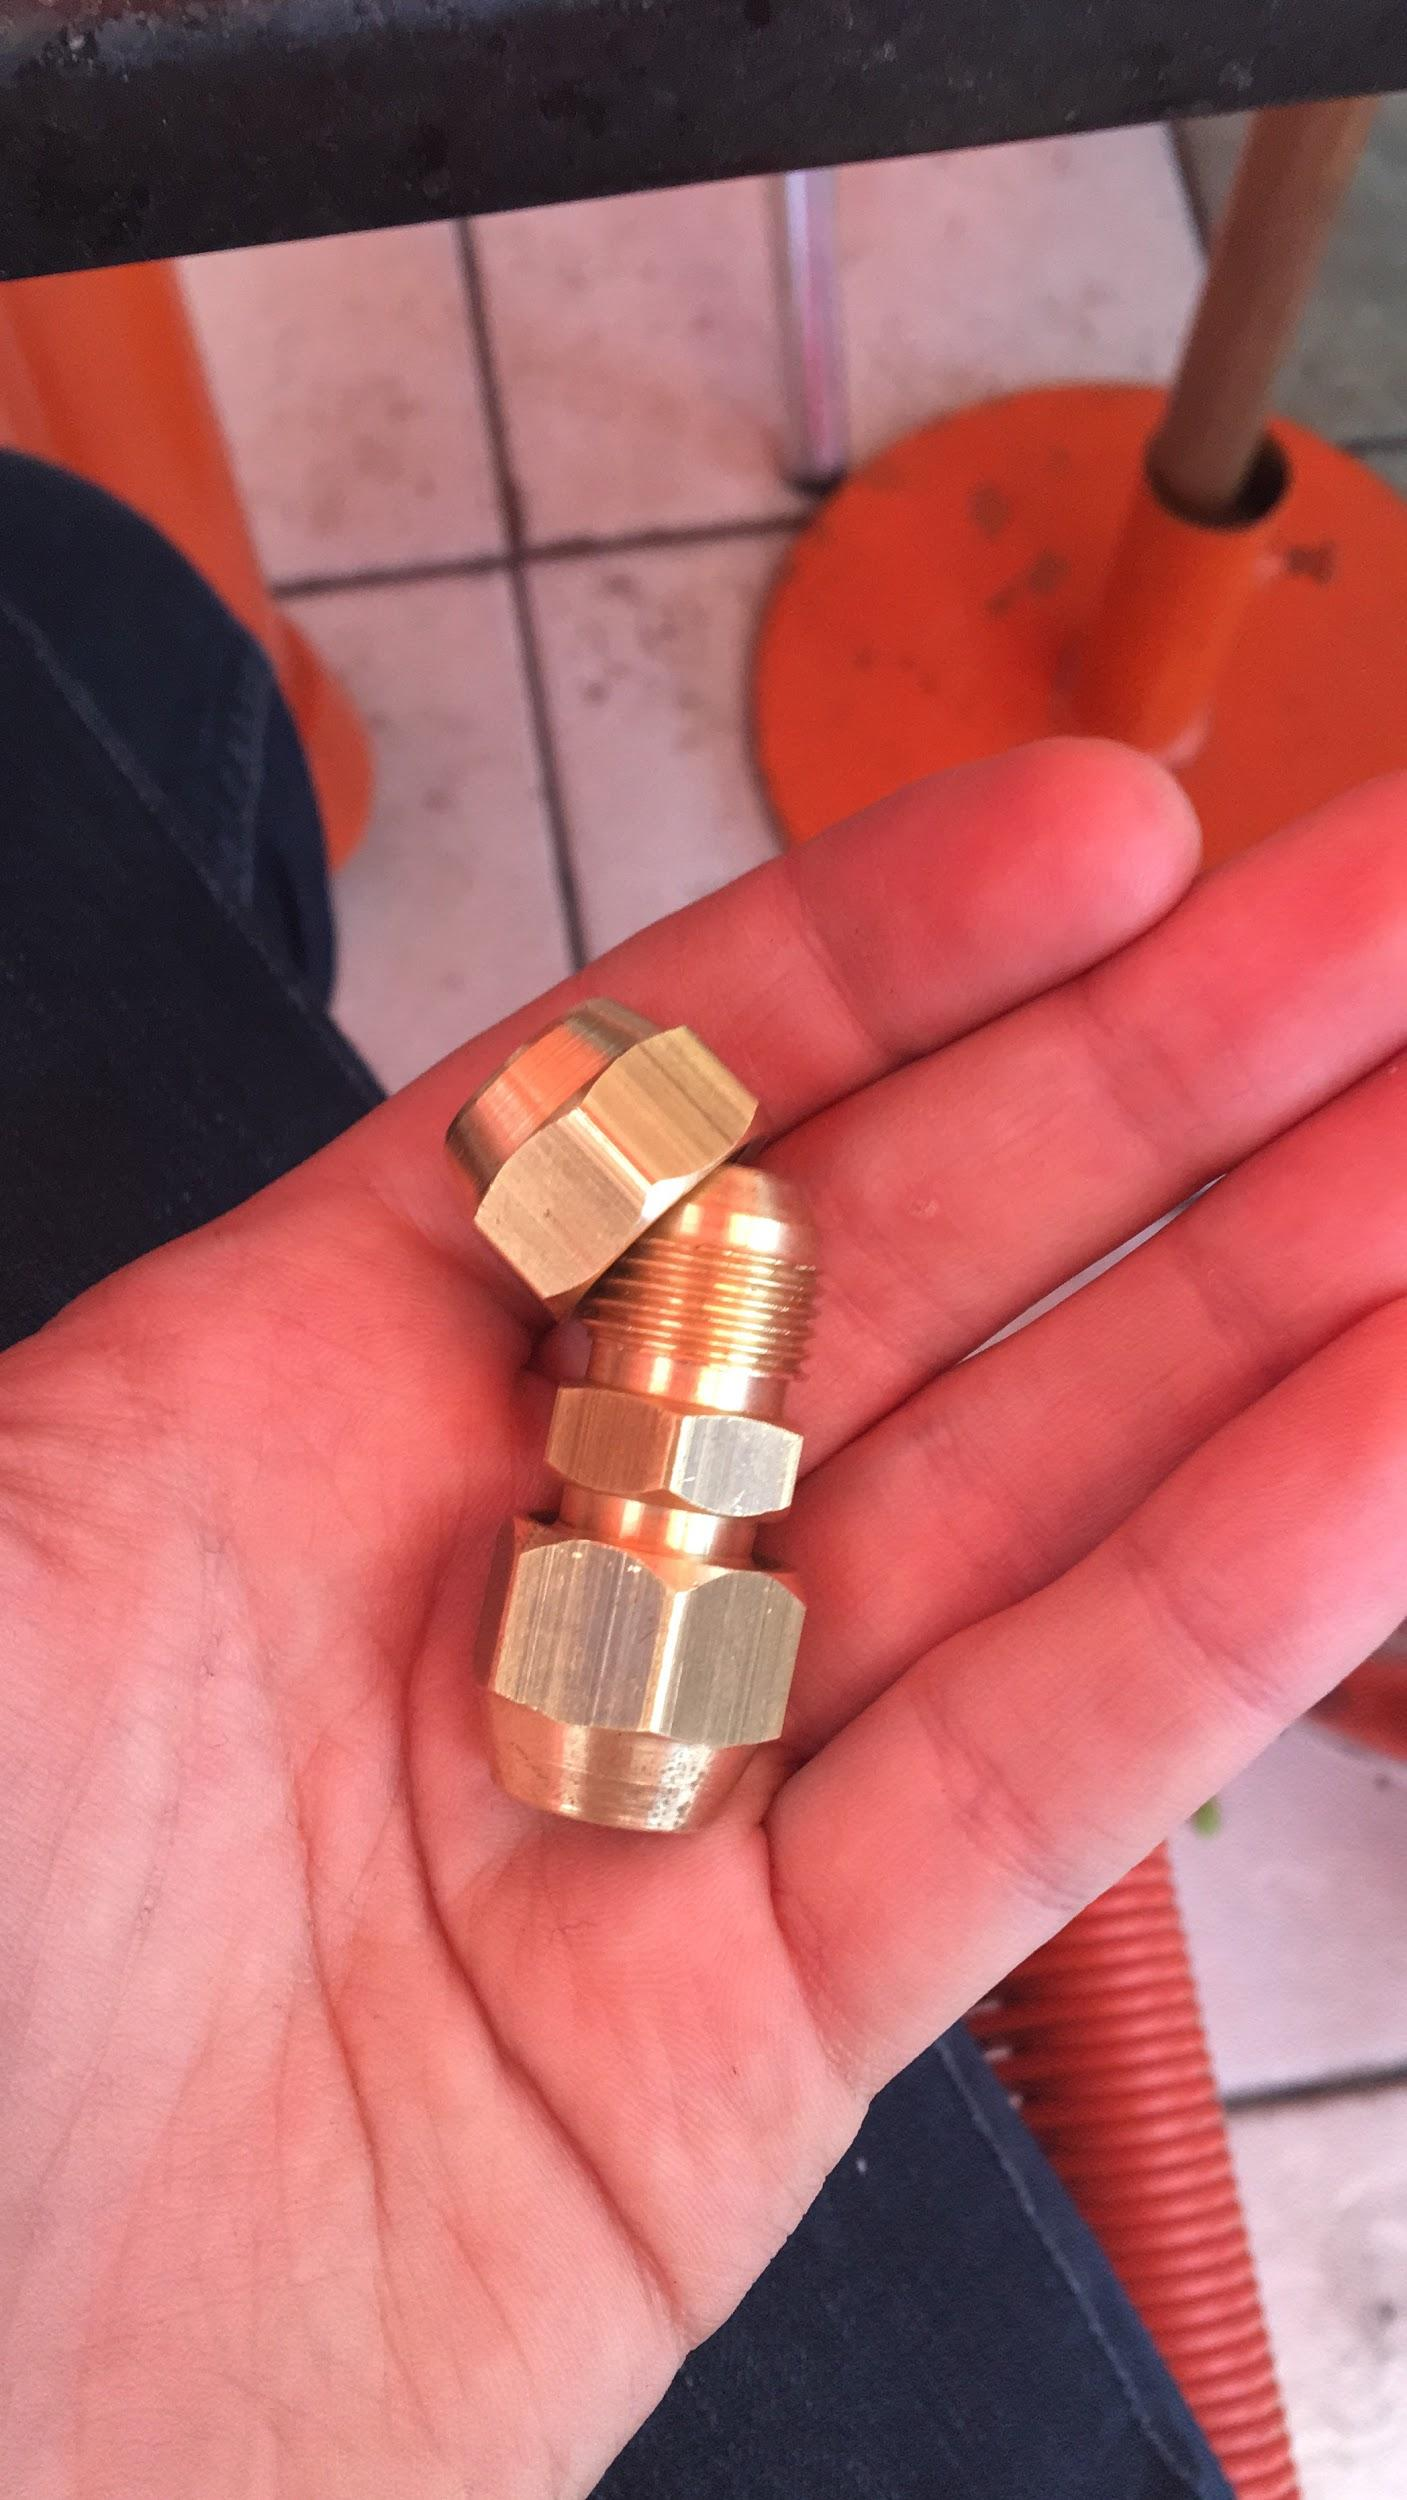
\includegraphics[scale= 0.2]{figuras/nipel-gas.png}
                            \caption{Nipel de gás. Fonte: Própria.}
                            \label{nipel-gas}
                        \end{figure}

                        Assim com a peça ilustrada acima realizou-se o processo de flangeamento dos tubos. Esse
                        processo consiste em alargar a espessura do tubo de cobre para que o tubo de alumínio
                        seja inserido e juntado pela peça acima não havendo vazamento de gás. O processo de
                        flangeamento e ilustrado na figura \ref{processo-flageamento}. 

                        \begin{figure}[!htb]
                            \centering
                            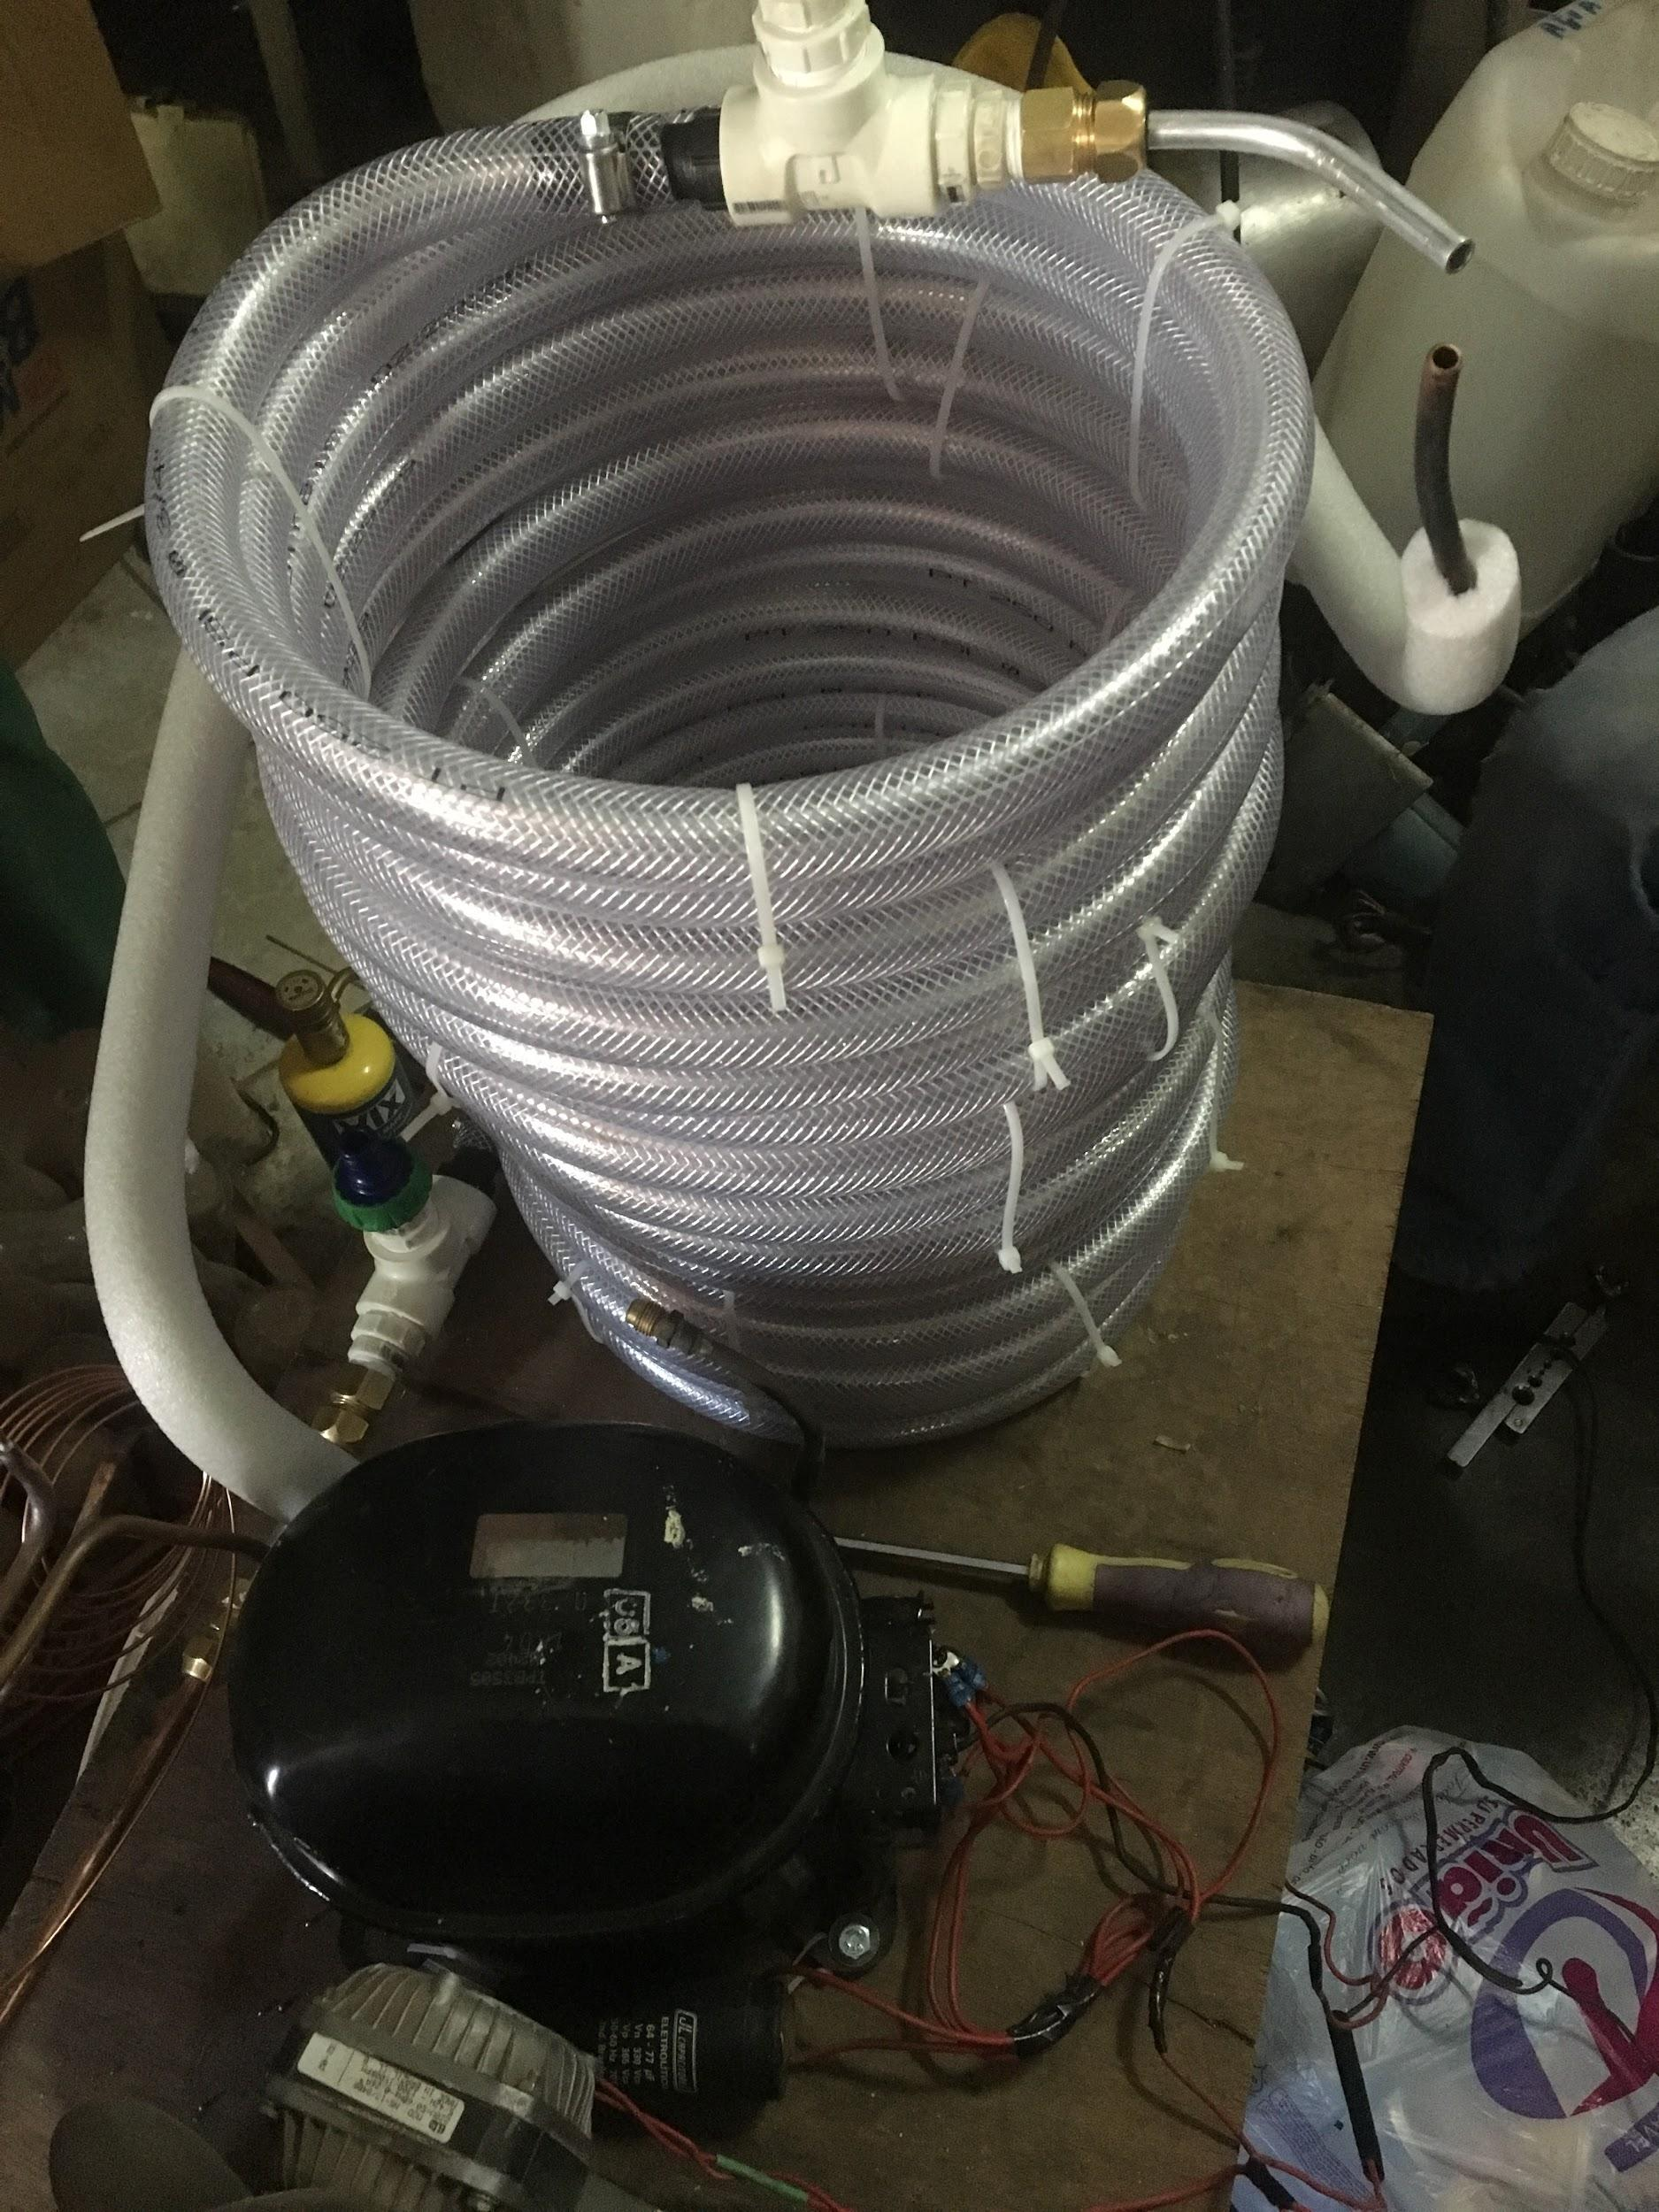
\includegraphics[scale= 0.2]{figuras/tubos-desconectados.png}
                            \caption{Tubos Desconectados. Fonte: Própria.}
                            \label{tubos-desconectados}
                        \end{figure}

                        \begin{figure}[!htb]
                            \centering
                            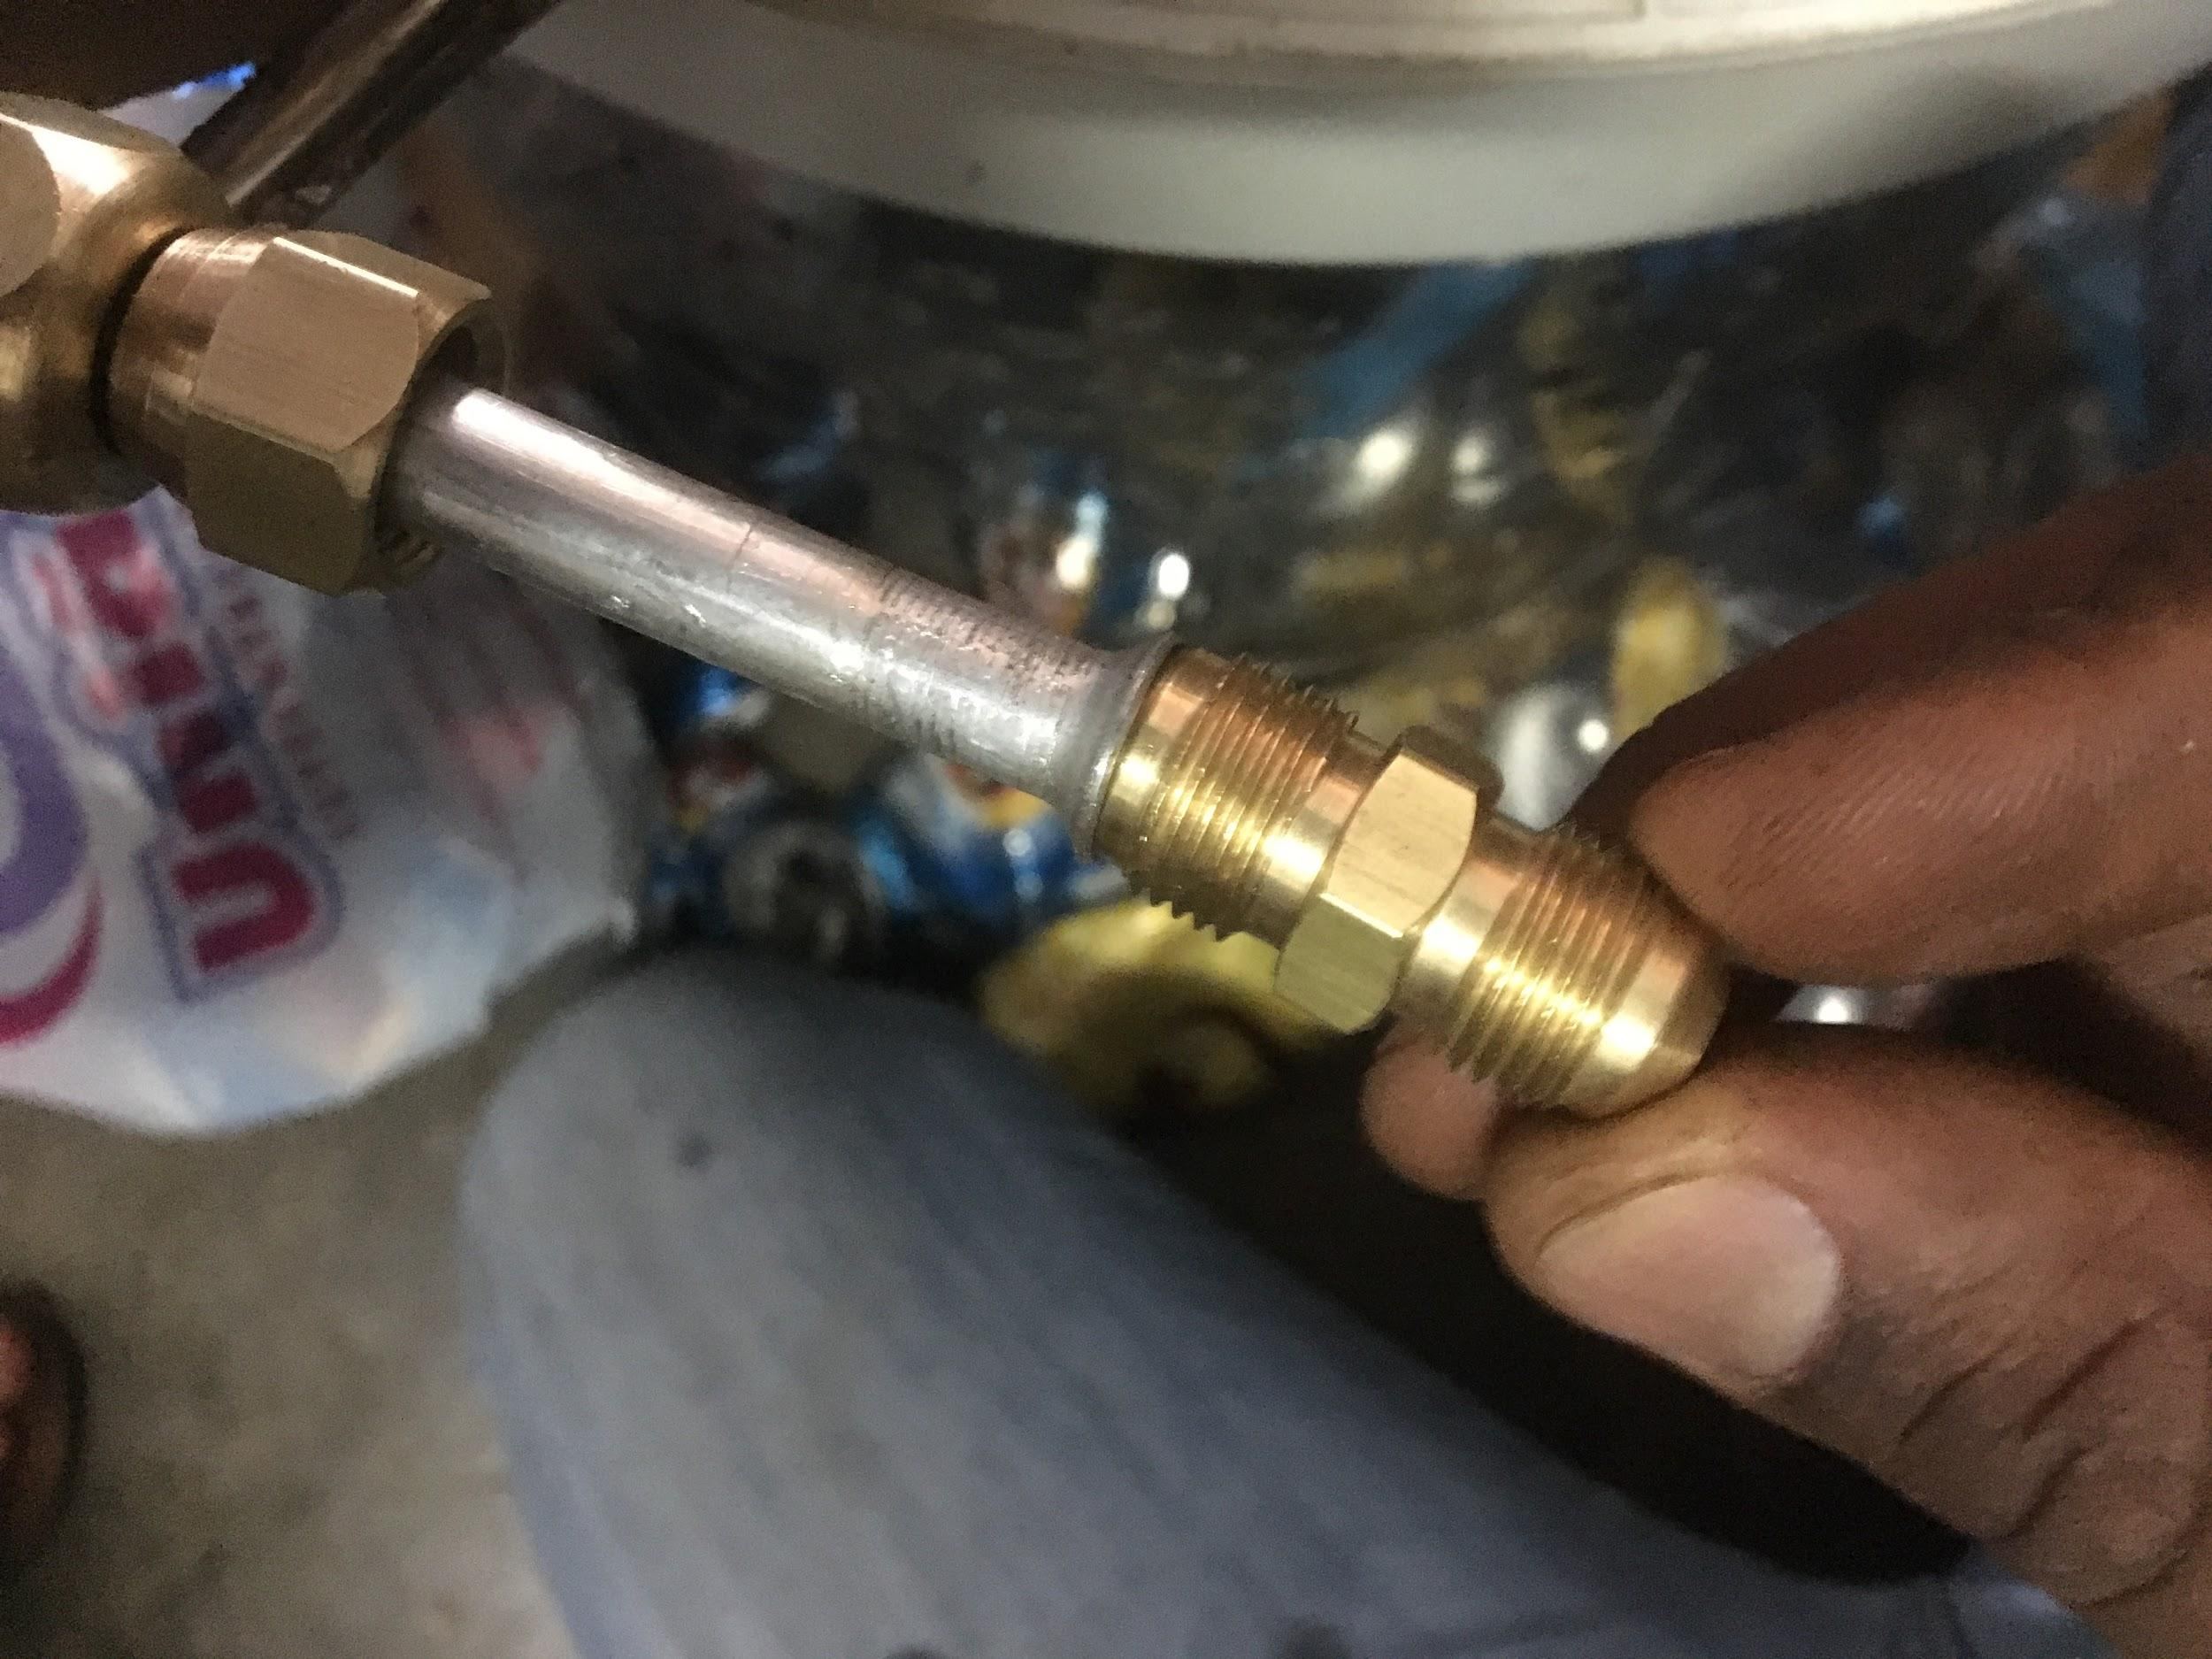
\includegraphics[scale= 0.2]{figuras/processo-flagelamento.png}
                            \caption{Processo de Flangeamento. Fonte: Própria.}
                            \label{processo-flageamento}
                        \end{figure}

                        Para a continuação da montagem do sistema, realizou-se a solda do tubo capilar
                        e filtro secador. Assim, com o sistema todo soldado e montado foi feita a
                        recarga de gás. Antes de abastecer o sistema, ligou-se o motocompressor para a
                        realização de uma câmara de vácuo dentro das tubulações. Depois dessa verificação
                        conectou-se o manifold nos diferentes pontos do sistema, parte de baixa e alta
                        pressão e conectou-se a mangueira de abastecimento permitindo a passagem de
                        fluido refrigerante. A carga foi realizada até que o sistema não suportasse
                        mais gás dentro desse. A figura abaixo mostra a recarga do sistema com o
                        fluido refrigerante R22. 

                        \begin{figure}[!htb]
                            \centering
                            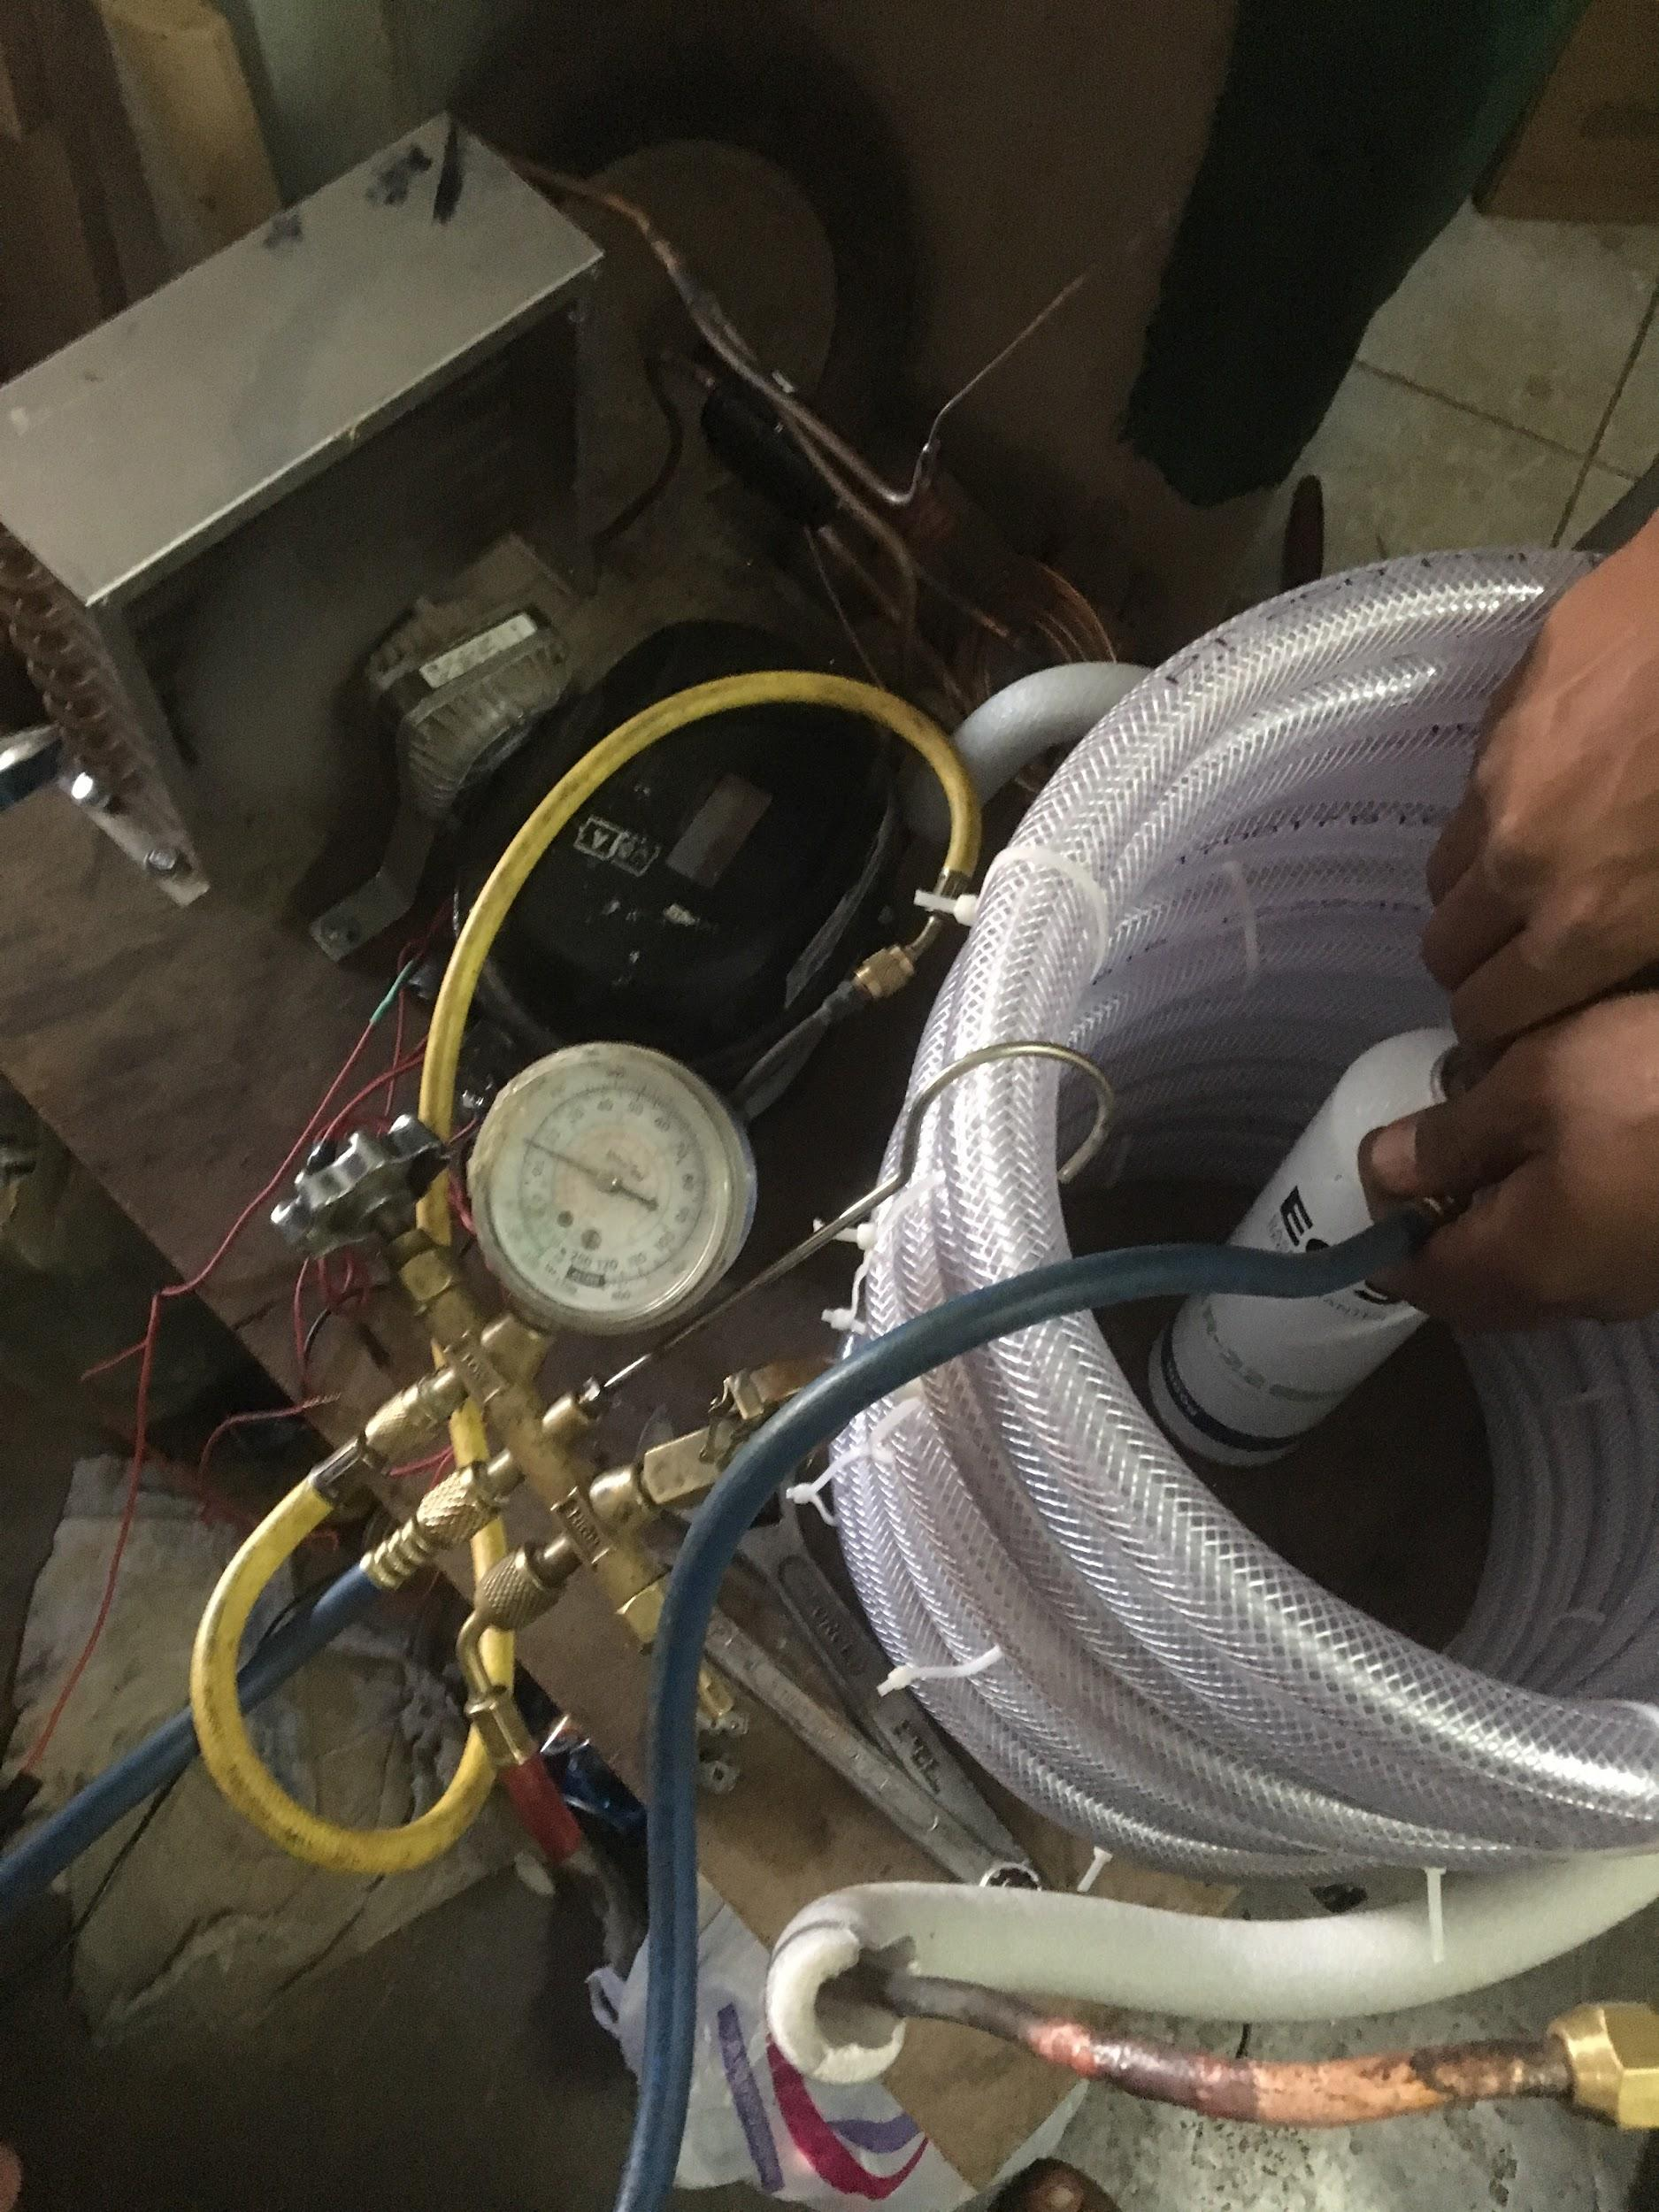
\includegraphics[scale= 0.2]{figuras/recarga-gas.png}
                            \caption{Recarga do sistema com gás R22. Fonte: Própria.}
                            \label{recarga-gas}
                        \end{figure}

                        Realizou-se os testes e notou-se que o condensador aplicado no sistema estava muito
                        pequeno para o evaporador escolhido. Assim sendo, repetiu-se todos os passos
                        acima quanto a soldagem dos tubos e a recarga de gás. Tendo assim o sistema de
                        refrigeração abaixo. 

                        COLOCAR FOTO BONITINHA DO SISTEMA 

                        Com o sistema pronto realizou-se testes e a partir desses montou-se a seguinte tabela
                        para o sistema de refrigeração: 

                        \begin{table}[H]
                            \centering
                            \caption{Testes Iniciais do Sistema de Refrigeração}
                            \label{testes-refrigeracao}
                            \begin{tabular}{|l|l|}
                                \hline
                                Capacidade Efetiva de Chopp & 2,5 Litros \\ \hline
                                Tempo de Aquecimento do Sistema &  \\ \hline
                                Tempo de Refrigeração &  \\ \hline
                            \end{tabular}
                        \end{table}
                        
    \section[Sistema de Proteção]{Sistema de Proteção}